\documentclass{article}

\usepackage{amsmath}
\usepackage{tikz}
\usepackage{parskip}
\usepackage{siunitx}
\usepackage{subcaption}

\newcommand{\del}[2]{\frac{\partial #1}{\partial #2}}  % Partial derivative
\newcommand{\deriv}[2]{\frac{\mathrm{d} #1}{\mathrm{d} #2}}  % Derivative
\newcommand{\dderiv}[2]{\frac{\mathrm{d}^2 #1}{\mathrm{d} #2^2}}  % Second derivative
\newcommand{\expval}[1]{\langle #1 \rangle}

\title{Exam Computational Physics\\
  2020}
\author{Thorvald M. Ballestad}

\begin{document}
\maketitle
\begin{abstract}
  Metropolis Monte Carlo simulation of 2D Ising model, using the Mon-Jasnow and extended Mon-Jasnow algorithm.
  This report is not intended as a scientific report, but as an answer to the exam.
  The goal of this report is to give a brief overview of how I have solved the problem, and then go into the parts of the solution that I think are the most interesting.
  Thus, this report consists of a brief documentation of the code and then explanations and thought on the interesting aspects of the solution.
\end{abstract}

\section{Overview of the code}
The simulation is written in Julia and the plots are generated in Python.
As the Python code is just simple plotting, I will not give it much focus here.
The code is separated into files, the main part being in \verb|utils.jl|.
Nothing should be run directly from \verb|utils.jl|, it contains the machinery that can be used from other designated scripts.
For each type of ``operation'' that we want to execute, there should exist a file, that extends \verb|utils.jl|, for example \verb|task1.jl| and \verb|investigate_error.jl|.


Metropolis: select at random -> attempt flip

Interesting solutions:
- Indexes for neighbor points
- Very modul based code.
  |-> Was very easy to implement new types of index vectors
- Does not really need energy, only the energy difference, which can be calulated explicitly every sweep
- Exponent lookup
- delta_H_sweep allocated outside loop
- Solution to ++ +- boundaries


\section{Results}


\begin{figure}[ht]
  \centering
  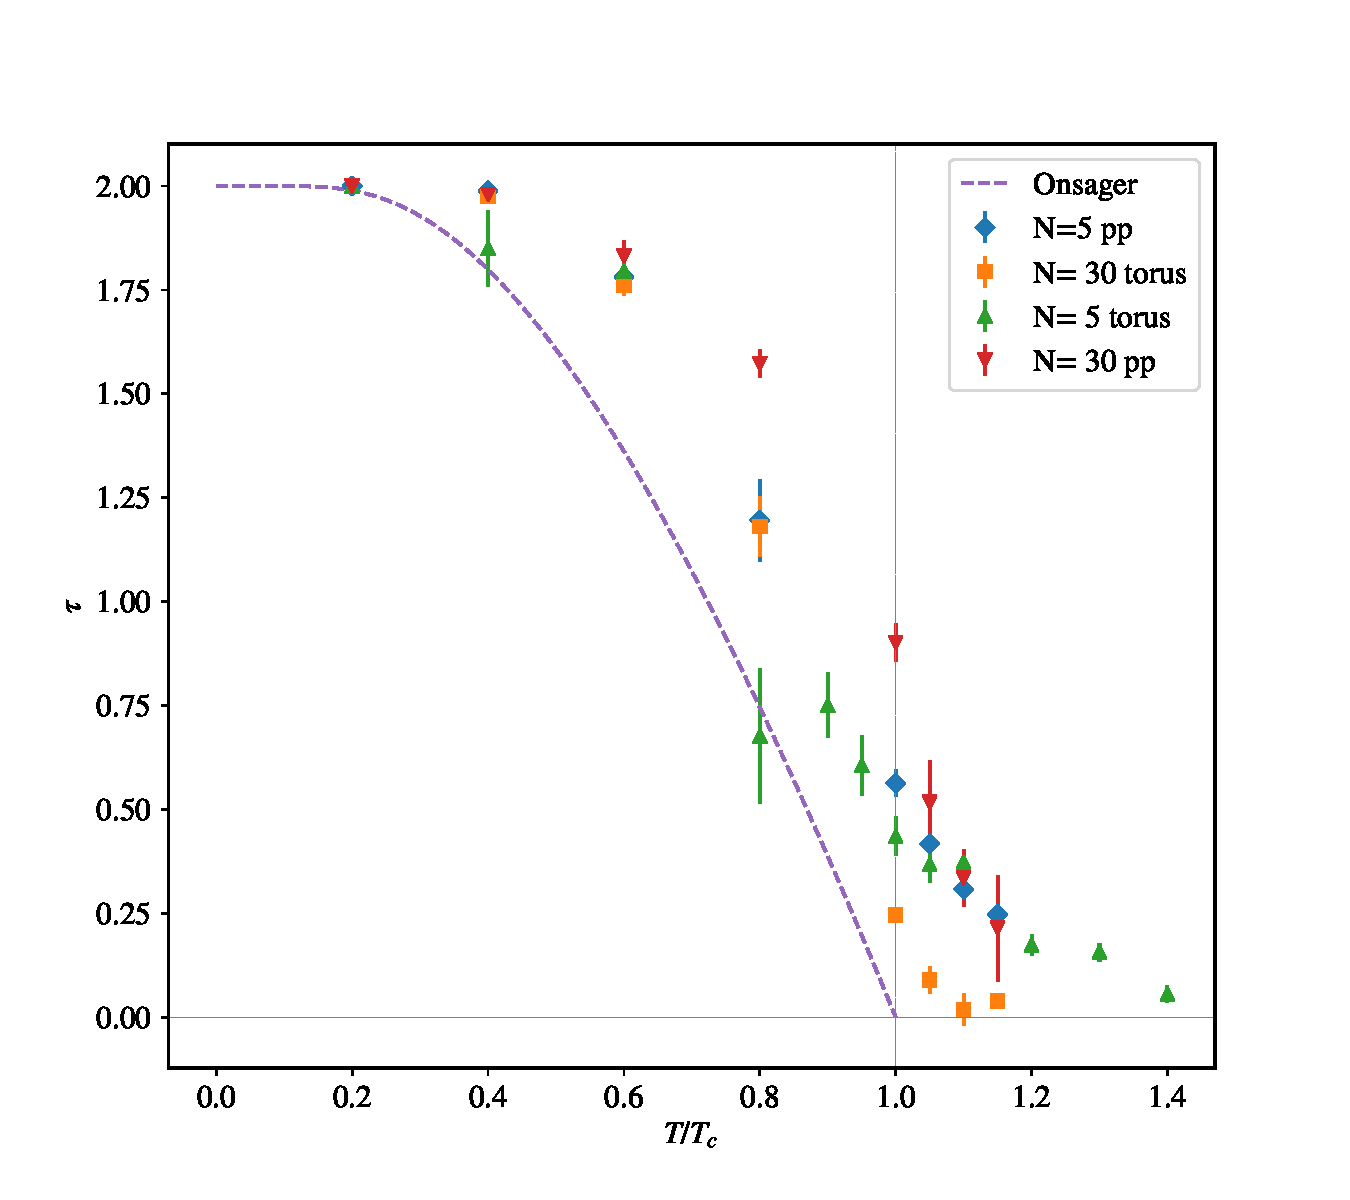
\includegraphics[width=.75\textwidth]{media/tau_T}
  \caption{$\tau$ as a function of T.\label{fig:tau_T}}
\end{figure}

\begin{figure}[ht]
  \centering
  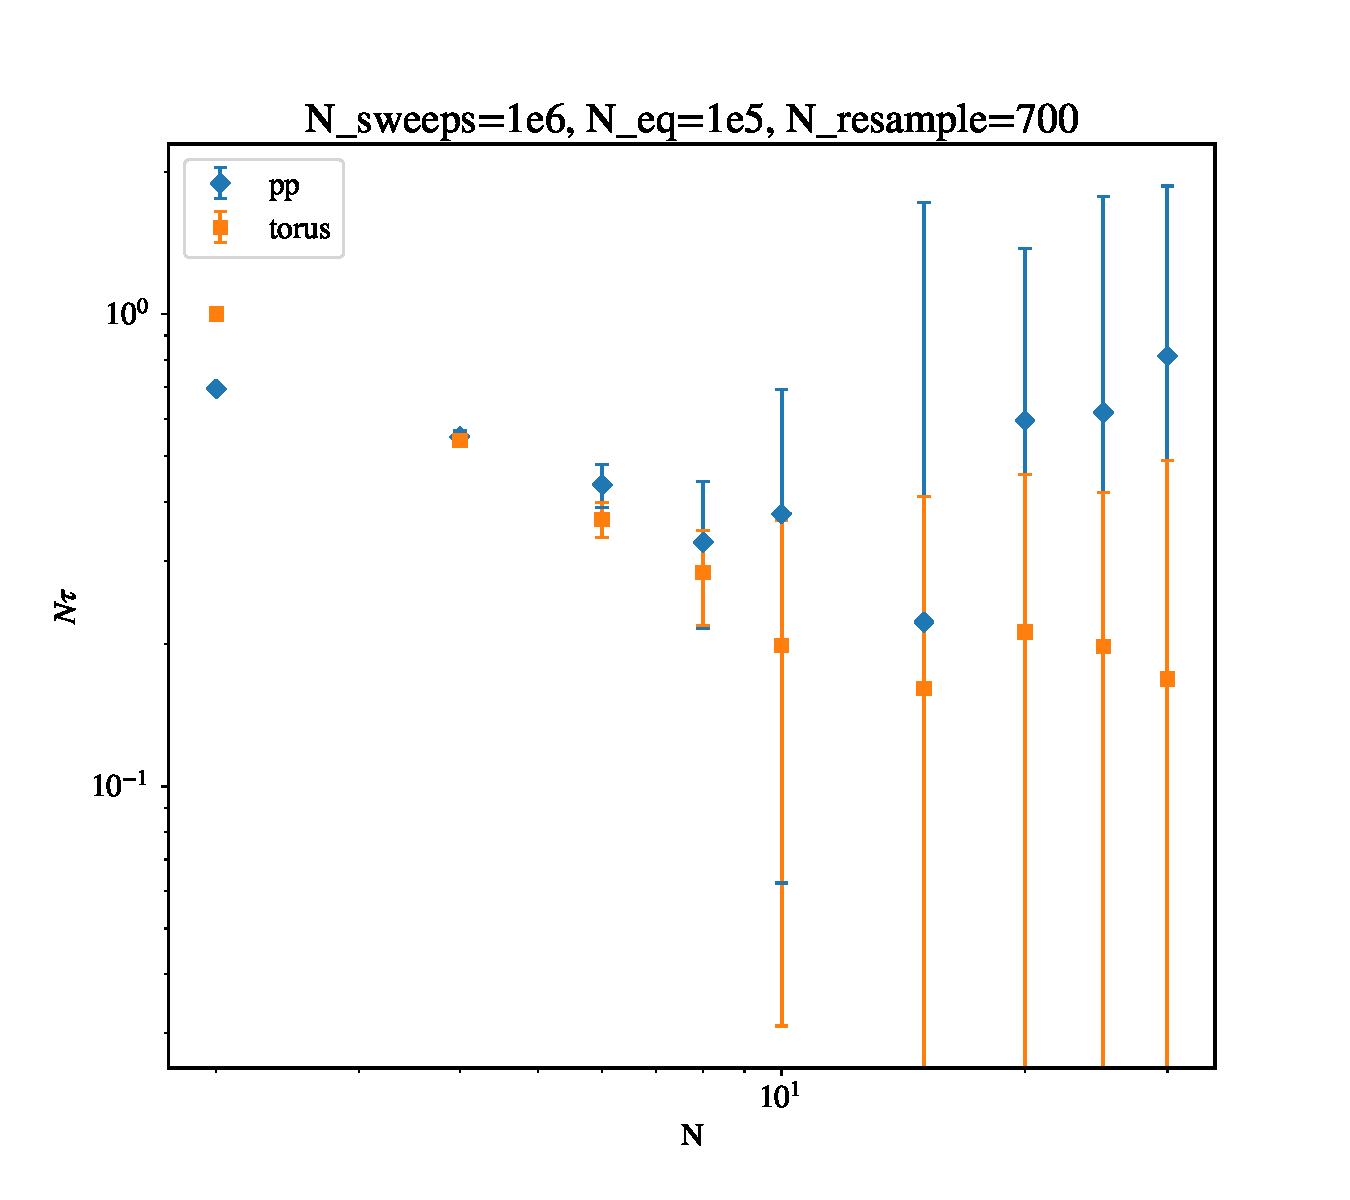
\includegraphics[width=.75\textwidth]{media/tau_N}
  \caption{$N\tau$ as a function of N for $T=T_c$.\label{fig:tau_N}}
\end{figure}

\begin{figure}[ht]
  \centering
  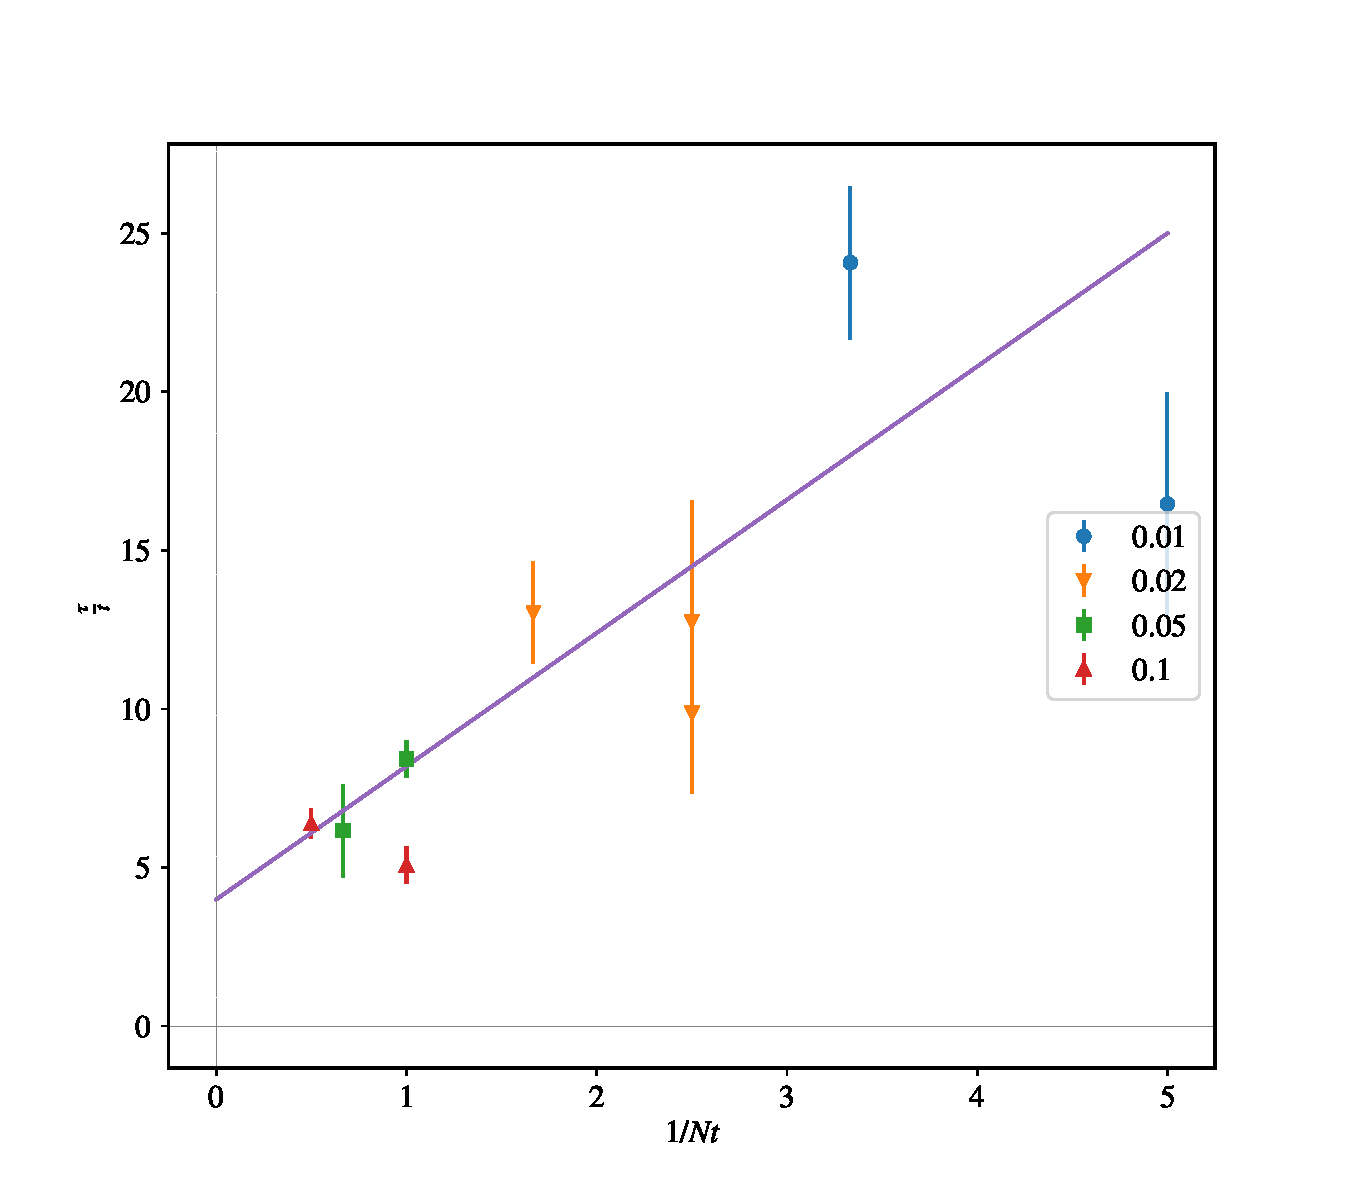
\includegraphics[width=.75\textwidth]{media/tau_TN}
  \caption{$\tau/t$ as a function of $\frac{1}{N t}$.\label{fig:tau_TN}}
\end{figure}


\section{Findings related to performance}
During the development process, several benchmarks were made, and I discovered some small changes that had huge impact on performance.
Especially pices of code that are involved in the very core of the simulation loop, the flipping, are vital to streamline as they are executed several million times.

- Index vectors, not having to create the tuples at the expense of using some more memory.
- UInt8 -> Integer, possibly some silent conversions that I did not find.
- Structs
- Optimizing neighbor funciton failed.
  |-> If one is able to optimize it, very advantegous.
- Neighbor sum
  |-> 30s -> 3.5s ( 1 hour -> 6 seconds of simulation )


\begin{thebibliography}{9}
\bibitem{niels} M. E. J. Newman and G. T. Barkema, \emph{Monte Carlo Methods in Statistical Physics} chap. 3, Oxford University Press, Oxford, 1999.

\bibitem{onsager}  L. Onsager, \emph{Crystal statistics. I. A two-dimensional model with an order-disorder transition},  Phys. Rev. 65, 117 (1944).

\bibitem{mon_jasnow} ]  K.K. Mon and D. Jasnow, \emph{Direct calculation of interfacial tension for lattice models by the Monte Carlo method}, Phys. Rev. A 30, 670 (1984). 
\end{thebibliography}
\end{document}
